%%%%%%%%%%%%%%%%%%%%%%%%%%%%%%%%%%%%%%%%%
% Beamer Presentation
% LaTeX Template
% Version 1.0 (10/11/12)
%
% This template has been downloaded from:
% http://www.LaTeXTemplates.com
%
% License:
% CC BY-NC-SA 3.0 (http://creativecommons.org/licenses/by-nc-sa/3.0/)
%
%%%%%%%%%%%%%%%%%%%%%%%%%%%%%%%%%%%%%%%%%

%----------------------------------------------------------------------------------------
%	PACKAGES AND THEMES
%----------------------------------------------------------------------------------------

\documentclass{beamer}

\mode<presentation> {
\usetheme{Madrid}
}
\setbeamertemplate{navigation symbols}{}

\usepackage{graphicx} % Allows including images
\usepackage{booktabs} % Allows the use of \toprule, \midrule and \bottomrule in tables
\usepackage{adjustbox}
\usepackage{amsmath}               % great math stuff
\usepackage{amsfonts}              % for blackboard bold, etc
\usepackage{amsthm}                % better theorem environments

\title[Effect of Authoritarian Legislature]{The Effect of Authoritarian Legislature on Regime-Opposition Interaction} % The short title appears at the bottom of every slide, the full title is only on the title page

\author{Anh Le} % Your name
\institute[Duke] % Your institution as it will appear on the bottom of every slide, may be shorthand to save space
{Duke University \\ % Your institution for the title page
\medskip
\textit{anh.le@duke.edu} % Your email address
}
\date{\today} % Date, can be changed to a custom date

\begin{document}
\setbeamercovered{transparent}

\begin{frame}
\titlepage % Print the title page as the first slide
\end{frame}

\section{Motivation}
\begin{frame}
\frametitle{Motivation}
\centering
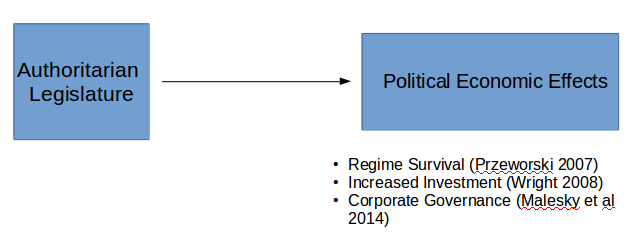
\includegraphics[width=0.8\textwidth]{legislature_to_pe}
\end{frame}

\begin{frame}
\frametitle{Motivation}
\centering
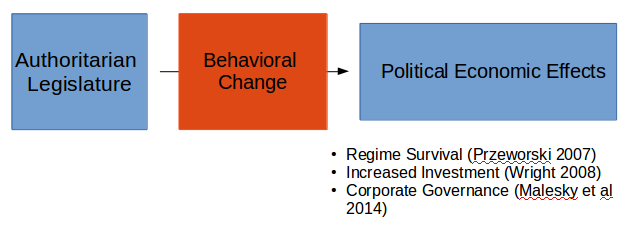
\includegraphics[width=0.8\textwidth]{legislature_to_behavior}
\end{frame}

\begin{frame}
\frametitle{Overview}
\tableofcontents
\end{frame}

\AtBeginSection[]
{
   \begin{frame}
       \frametitle{Outline}
       \tableofcontents[currentsection]
   \end{frame}
}

\section{The Argument}

\begin{frame}
\frametitle{The Argument}
\begin{itemize}
\item<1-> Theory: Authoritarian legislature provides information, raises cost of violence, and enables side payment. Given these conditions, negotiated peace is more likely than costly violence
\item<2-> Empirical (experimental): A survey vignette experiment that prime Vietnamese businesses to think about the inclusion of businessmen in Vietnam National Assembly. Test whether businesses are more willing to participate in the legislature when primed
\item<3-> Empirical (large-n): Use event data to examine violence in regime-dissident interaction. Use matched panels to construct better counter-factual
\end{itemize}
\end{frame}

%------------------------------------------------

\section{Theory}
\begin{frame}
\frametitle{Regime-Opposition Bargaining Game}
\begin{itemize}
\item Violence is the final arbiter in authoritarian politics
\item Regime-opposition interaction is best modeled as a bargaining game, similar to the bargain between two sovereign states with the option of going to war (Fearon 1995)
\end{itemize}
\end{frame}

\begin{frame}
\frametitle{Regime-Opposition Bargaining Game}
\centering
\begin{itemize}
\item Negotiation about the share $x$ ($0 < x < 1$) of a good given to the opposition
\item Violence costs the autocrat $c_A$ and the opposition $c_O$
\item Expected utility depends on the probability of the opposition winning, $p$
\item<2-> Violence should never happen since $x$ that falls within the bargaining range $(p - c_O, p + c_A)$ is preferable to both sides
\end{itemize}
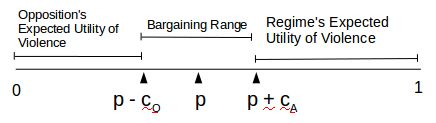
\includegraphics[width=0.7\textwidth]{general_model}
\end{frame}

\begin{frame}
\frametitle{The Model}
\centering
Violence can still happen if there is:
\begin{itemize}
\item Information asymmetry regarding $p$ leading to non-overlapping bargaining ranges
\only<1>{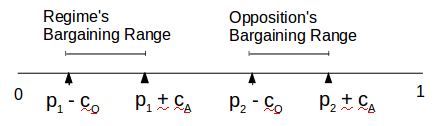
\includegraphics[width=0.8\textwidth]{information_asymmetry}}
\item<2-> The bargaining range $(p - c_O, p + c_A)$ is too small
\only<2>{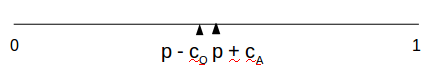
\includegraphics[width=0.8\textwidth]{small_range}}
\item<3-> Unit indivisibility
\only<3>{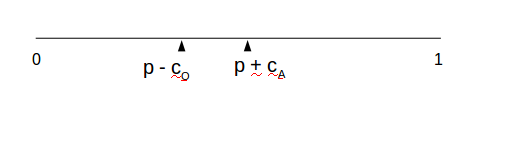
\includegraphics[width=0.8\textwidth]{unit_indivisibility}}
\end{itemize}
\end{frame}

\begin{frame}
\frametitle{Regime-Opposition Bargaining Game}
However, authoritarian legislature solves all of these issues
\begin{itemize}
\item<1> (Information Asymmetry) Elections and legislative session provide information about both sides' capacity
\item<2> (Small Bargaining Range) Cost of violent uprising and repression is increased relative to negotiation
\item<3> (Unit indivisibility) Negotiations over multiple issues in the legislature enable side payments
\end{itemize}
\end{frame}
\section{Experimental Design}

\begin{frame}
\frametitle{Business in Vietnam}
\end{frame}

\begin{frame}
\frametitle{Experimental Design}

(Control prompt) We want to understand how business participate in the process of economic policy making\\~\\

(Treatment prompt) We want to understand how business participate in the process of economic policy making, \textit{especially since the National Assembly has recently included more delegates that are businessmen} (emphasis added)\\~\\

Question: Is approaching National Assembly delegates to express opinions about economic polices effective or not?

\end{frame}

\begin{frame}
\frametitle{Checking Experimental Assumption}
\centering
\begin{itemize}
\item<1-2> Balance between the Treated and the Control
\item<3> Same response rate between the Treated and the Control
\item<4-5> Balance between Respondents and Non-Respondents
\end{itemize}
\begin{columns}[T] % align columns
\begin{column}{.48\textwidth}
\only<2,5>{\adjustbox{max height=0.3\textheight,
           max width=\textwidth}{
\begin{tabular}{rrrrl}
  \hline
 & Mean treated & Mean control & p-value &   \\ 
  \hline
Limited Liability & 0.54 & 0.57 & 0.09 & * \\ 
  Joint Stock & 0.23 & 0.23 & 0.84 &  \\ 
  Partnership & 0.00 & 0.00 & 0.38 &  \\ 
  Other form of ownership & 0.01 & 0.00 & 0.03 & ** \\ 
  Manufacturing & 0.08 & 0.09 & 0.57 &  \\ 
  Construction & 0.28 & 0.27 & 0.93 &  \\ 
  Service & 0.66 & 0.67 & 0.47 &  \\ 
  Agriculture & 0.10 & 0.08 & 0.01 & ** \\ 
  Mining & 0.02 & 0.03 & 0.09 & * \\ 
  Revenue (0.5-1 billion VND) & 0.22 & 0.22 & 0.98 &  \\ 
  Revenue (1-5 billion VND) & 0.43 & 0.43 & 0.71 &  \\ 
  Revenue (5-10 billion VND) & 0.07 & 0.08 & 0.23 &  \\ 
  Revenue (10-50 billion VND) & 0.05 & 0.06 & 0.39 &  \\ 
  Revenue (50-200 billion VND) & 0.01 & 0.01 & 0.94 &  \\ 
  Revenue (200-500 billion VND) & 0.00 & 0.00 & 0.81 &  \\ 
  Revenue (above 500 billion VND) & 0.00 & 0.00 & 0.53 &  \\ 
  Size (5-9 people) & 0.36 & 0.34 & 0.12 &  \\ 
  Size (10-49 people) & 0.21 & 0.24 & 0.05 & ** \\ 
  Size (50-199 people) & 0.06 & 0.05 & 0.49 &  \\ 
  Size (200-299 people) & 0.01 & 0.01 & 0.58 &  \\ 
  Size (300-499 people) & 0.00 & 0.00 & 0.20 &  \\ 
  Size (500-1000 people) & 0.00 & 0.00 & 0.81 &  \\ 
  Size (more than 1000 people) & 0.00 & 0.00 & 0.08 & * \\ 
  Main customer (State) & 0.19 & 0.19 & 0.57 &  \\ 
  Main customer (Private) & 0.58 & 0.62 & 0.02 & ** \\ 
  Main customer (Foreign in VN) & 0.05 & 0.04 & 0.33 &  \\ 
  Main customer (Foreign, direct) & 0.03 & 0.03 & 0.25 &  \\ 
  Main customer (Foreign, indirect) & 0.02 & 0.01 & 0.14 &  \\ 
  Equitized local state-owned enterprise & 0.05 & 0.06 & 0.21 &  \\ 
  Equitized central state-owned enterprise & 0.01 & 0.01 & 0.28 &  \\ 
  Firm with some state-owned equities & 0.03 & 0.02 & 0.26 &  \\ 
  Firm that was formerly household business & 0.74 & 0.73 & 0.24 &  \\ 
  Firm with shares listed & 0.01 & 0.00 & 0.39 &  \\ 
  Firm owner graduated from university & 0.62 & 0.63 & 0.91 &  \\ 
  Firm owner with MBA & 0.03 & 0.04 & 0.45 &  \\ 
  Firm owner was a leader of a State agency & 0.04 & 0.03 & 0.37 &  \\ 
  Firm owner was a military officer & 0.05 & 0.04 & 0.26 &  \\ 
  Firm owner was a manager of SOE & 0.13 & 0.12 & 0.22 &  \\ 
  Firm owner was an employee at SOE & 0.15 & 0.15 & 0.87 &  \\ 
   \hline
\end{tabular}       
}}
\end{column}%
\begin{column}{.48\textwidth}
\only<5>{\adjustbox{max height=0.3\textheight,
           max width=\textwidth}{
\begin{tabular}{rrrrl}
  \hline
 & Mean (resp) & Mean (non-resp) & p-value &   \\ 
  \hline
Limited Liability & 0.55 & 0.56 & 0.81 &  \\ 
  Joint Stock & 0.23 & 0.20 & 0.01 & ** \\ 
  Partnership & 0.00 & 0.00 & 0.75 &  \\ 
  Other form of ownership & 0.00 & 0.00 & 0.04 & ** \\ 
  Manufacturing & 0.09 & 0.08 & 0.42 &  \\ 
  Construction & 0.27 & 0.24 & 0.00 & *** \\ 
  Service & 0.67 & 0.68 & 0.15 &  \\ 
  Agriculture & 0.09 & 0.07 & 0.00 & *** \\ 
  Mining & 0.02 & 0.02 & 0.03 & ** \\ 
  Revenue (0.5-1 billion VND) & 0.22 & 0.22 & 0.98 &  \\ 
  Revenue (1-5 billion VND) & 0.43 & 0.41 & 0.20 &  \\ 
  Revenue (5-10 billion VND) & 0.08 & 0.08 & 0.84 &  \\ 
  Revenue (10-50 billion VND) & 0.05 & 0.05 & 0.91 &  \\ 
  Revenue (50-200 billion VND) & 0.01 & 0.01 & 0.52 &  \\ 
  Revenue (200-500 billion VND) & 0.00 & 0.00 & 0.85 &  \\ 
  Revenue (above 500 billion VND) & 0.00 & 0.00 & 0.26 &  \\ 
  Size (5-9 people) & 0.35 & 0.33 & 0.15 &  \\ 
  Size (10-49 people) & 0.22 & 0.23 & 0.77 &  \\ 
  Size (50-199 people) & 0.06 & 0.05 & 0.24 &  \\ 
  Size (200-299 people) & 0.01 & 0.01 & 0.93 &  \\ 
  Size (300-499 people) & 0.00 & 0.00 & 0.43 &  \\ 
  Size (500-1000 people) & 0.00 & 0.00 & 0.96 &  \\ 
  Size (more than 1000 people) & 0.00 & 0.00 & 0.67 &  \\ 
  Main customer (State) & 0.19 & 0.17 & 0.02 & ** \\ 
  Main customer (Private) & 0.60 & 0.63 & 0.01 & ** \\ 
  Main customer (Foreign in VN) & 0.04 & 0.04 & 0.96 &  \\ 
  Main customer (Foreign, direct) & 0.03 & 0.03 & 0.85 &  \\ 
  Main customer (Foreign, indirect) & 0.01 & 0.01 & 0.78 &  \\ 
  Equitized local state-owned enterprise & 0.06 & 0.05 & 0.35 &  \\ 
  Equitized central state-owned enterprise & 0.01 & 0.01 & 0.60 &  \\ 
  Firm with some state-owned equities & 0.03 & 0.02 & 0.52 &  \\ 
  Firm that was formerly household business & 0.73 & 0.70 & 0.00 & ** \\ 
  Firm with shares listed & 0.00 & 0.00 & 0.78 &  \\ 
  Firm owner graduated from university & 0.63 & 0.58 & 0.00 & *** \\ 
  Firm owner with MBA & 0.04 & 0.03 & 0.06 & * \\ 
  Firm owner was a leader of a State agency & 0.04 & 0.03 & 0.04 & ** \\ 
  Firm owner was a military officer & 0.05 & 0.04 & 0.12 &  \\ 
  Firm owner was a manager of SOE & 0.12 & 0.11 & 0.03 & ** \\ 
  Firm owner was an employee at SOE & 0.15 & 0.14 & 0.48 &  \\ 
   \hline
\end{tabular}          
}}
\end{column}%
\end{columns}
\end{frame}

\begin{frame}
\frametitle{Covariate Balance: Respondent vs Non-respondents}
\framezoom<1><2>[border=1](0cm,6.1cm)(7cm,1.5cm)
\adjustbox{max height=\dimexpr\textheight-5.5cm\relax,
           max width=\textwidth}{
\begin{tabular}{rrrrl}
  \hline
 & Mean (resp) & Mean (non-resp) & p-value &   \\ 
  \hline
Limited Liability & 0.55 & 0.56 & 0.81 &  \\ 
  Joint Stock & 0.23 & 0.20 & 0.01 & ** \\ 
  Partnership & 0.00 & 0.00 & 0.75 &  \\ 
  Other form of ownership & 0.00 & 0.00 & 0.04 & ** \\ 
  Manufacturing & 0.09 & 0.08 & 0.42 &  \\ 
  Construction & 0.27 & 0.24 & 0.00 & *** \\ 
  Service & 0.67 & 0.68 & 0.15 &  \\ 
  Agriculture & 0.09 & 0.07 & 0.00 & *** \\ 
  Mining & 0.02 & 0.02 & 0.03 & ** \\ 
  Revenue (0.5-1 billion VND) & 0.22 & 0.22 & 0.98 &  \\ 
  Revenue (1-5 billion VND) & 0.43 & 0.41 & 0.20 &  \\ 
  Revenue (5-10 billion VND) & 0.08 & 0.08 & 0.84 &  \\ 
  Revenue (10-50 billion VND) & 0.05 & 0.05 & 0.91 &  \\ 
  Revenue (50-200 billion VND) & 0.01 & 0.01 & 0.52 &  \\ 
  Revenue (200-500 billion VND) & 0.00 & 0.00 & 0.85 &  \\ 
  Revenue (above 500 billion VND) & 0.00 & 0.00 & 0.26 &  \\ 
  Size (5-9 people) & 0.35 & 0.33 & 0.15 &  \\ 
  Size (10-49 people) & 0.22 & 0.23 & 0.77 &  \\ 
  Size (50-199 people) & 0.06 & 0.05 & 0.24 &  \\ 
  Size (200-299 people) & 0.01 & 0.01 & 0.93 &  \\ 
  Size (300-499 people) & 0.00 & 0.00 & 0.43 &  \\ 
  Size (500-1000 people) & 0.00 & 0.00 & 0.96 &  \\ 
  Size (more than 1000 people) & 0.00 & 0.00 & 0.67 &  \\ 
  Main customer (State) & 0.19 & 0.17 & 0.02 & ** \\ 
  Main customer (Private) & 0.60 & 0.63 & 0.01 & ** \\ 
  Main customer (Foreign in VN) & 0.04 & 0.04 & 0.96 &  \\ 
  Main customer (Foreign, direct) & 0.03 & 0.03 & 0.85 &  \\ 
  Main customer (Foreign, indirect) & 0.01 & 0.01 & 0.78 &  \\ 
  Equitized local state-owned enterprise & 0.06 & 0.05 & 0.35 &  \\ 
  Equitized central state-owned enterprise & 0.01 & 0.01 & 0.60 &  \\ 
  Firm with some state-owned equities & 0.03 & 0.02 & 0.52 &  \\ 
  Firm that was formerly household business & 0.73 & 0.70 & 0.00 & ** \\ 
  Firm with shares listed & 0.00 & 0.00 & 0.78 &  \\ 
  Firm owner graduated from university & 0.63 & 0.58 & 0.00 & *** \\ 
  Firm owner with MBA & 0.04 & 0.03 & 0.06 & * \\ 
  Firm owner was a leader of a State agency & 0.04 & 0.03 & 0.04 & ** \\ 
  Firm owner was a military officer & 0.05 & 0.04 & 0.12 &  \\ 
  Firm owner was a manager of SOE & 0.12 & 0.11 & 0.03 & ** \\ 
  Firm owner was an employee at SOE & 0.15 & 0.14 & 0.48 &  \\ 
   \hline
\end{tabular}          
}
\end{frame}

\begin{frame}
\frametitle{Experimental Result}
\begin{table}
\begin{tabular}{@{\extracolsep{5pt}}lc} 
\\[-1.8ex]\hline 
\hline \\[-1.8ex] 
 & \multicolumn{1}{c}{\textit{Dependent variable:}} \\ 
\cline{2-2} 
\\[-1.8ex] & Contacting the National Assembly is effective \\ 
\hline \\[-1.8ex] 
 Treatment prompt & 0.264$^{***}$ \\ 
  & (0.073) \\ 
  & \\ 
 Constant & 0.929$^{***}$ \\ 
  & (0.049) \\ 
  & \\ 
\hline \\[-1.8ex] 
Observations & 3,951 \\ 
Log Likelihood & $-$2,253.137 \\ 
Akaike Inf. Crit. & 4,510.274 \\ 
\hline 
\hline \\[-1.8ex] 
\textit{Note:}  & \multicolumn{1}{r}{$^{*}$p$<$0.1; $^{**}$p$<$0.05; $^{***}$p$<$0.01} \\ 
\end{tabular} 
\end{table}
\end{frame}

\section{Large-N event data analysis}
\begin{frame}
\frametitle{Description of Data}
\begin{itemize}
\item Independent variable (\textit{legislature}): multiple parties are legal
\item Dependent variable (\textit{violence}): event data from news report, recording individual regime-opposition interaction. Violence is measured by the Goldstein scale (-10 to 10)
\end{itemize}
\end{frame}

\begin{frame}
\frametitle{Empirical Strategy}
\begin{itemize}
\item Create short panels of four country years
\item Treatment panel: no legislature in the first year, legislature in the next three years
\item Control panel: no legislature throughout the panel
\item Match panels based on the co-variates of the first years
\end{itemize}
\end{frame}

\begin{frame}
\frametitle{Matching Result}
\centering
\adjustbox{max height=\dimexpr\textheight-5.5cm\relax,
           max width=\textwidth}{
\begin{tabular}{lrrlrrrl}
  \hline
 & \multicolumn{3}{c}{Pre-Match} &   \multicolumn{3\textbf{}}{c}{Post-Match} \\
Covariate & Treated & Control & p-value & Treated & Control & p-value &  \\ 
  \hline
Ethnic Fractionalization & 0.61 & 0.59 & 0.59 & 0.61 & 0.60 & 0.81 &  \\ 
Violence (Goldstein score) & -4.50 & -4.05 & 0.51 & -4.50 & -4.49 & 0.94 &  \\ 
$\text{Violence}^2$ & 29.84 & 23.22 & 0.34 & 29.84 & 29.03 & 0.65 &  \\ 
Regime duration (years) & 12.08 & 34.30 & 0.00*** & 12.08 & 12.71 & 0.71 &  \\ 
$\text{Regime duration}^2$ & 278.00 & 2783.57 & 0.00** & 278.00 & 287.38 & 0.89 &  \\ 
Military & 0.08 & 0.06 & 0.67 & 0.08 & 0.12 & 0.57 &  \\ 
Monarchy & 0.04 & 0.25 & 0.00*** & 0.04 & 0.04 & 1.00 &  \\ 
Party & 0.29 & 0.48 & 0.07* & 0.29 & 0.29 & 1.00 &  \\ 
log(gdp) & 22.65 & 23.95 & 0.00*** & 22.65 & 22.78 & 0.67 &  \\ 
log(gdp per capita) & 7.63 & 8.58 & 0.00*** & 7.63 & 7.65 & 0.95 &  \\ 
Military expenditure (\%GDP) & 2.44 & 4.34 & 0.00*** & 2.44 & 2.40 & 0.89 &  \\
Land (1000 $\text{km}^2$)& 760.22 & 1674.68 & 0.00*** & 760.21 & 783.37 & 0.80 &  \\ 
Population (million) & 22.62 & 140.73 & 0.00*** & 22.62 & 21.74 & 0.90 &  \\
Resource Export (\%GDP) & 14.79 & 22.64 & 0.03** & 14.79 & 14.16 & 0.72 &  \\ 
Resource $\times$ Ethnic & 8.61 & 14.43 & 0.01** & 8.61 & 8.33 & 0.82 & \\
  \hline
\end{tabular}
}
\end{frame}

\begin{frame}
\frametitle{Matching Result}
\centering
\adjustbox{max height=\dimexpr\textheight-5.5cm\relax,
           max width=\textwidth}{
\begin{tabular}{lrlr}
  \hline
 \multicolumn{2}{c}{Treatment} &   \multicolumn{2}{c}{Control} \\
Country & Year & Country & Year \\ 
  \hline
Algeria & 1996 & Sudan & 1992 \\ 
  Angola & 1992 & Angola & 2000 \\ 
  Azerbaijan & 1992 & Uganda & 1991 \\ 
  Belarus & 2004 & Belarus & 2000 \\ 
  Cambodia & 1993 & Laos & 1999 \\ 
  Central African Republic & 2005 & Uganda & 2001 \\ 
  Chad & 1997 & Central African Republic & 1992 \\ 
  Congo, Republic & 2002 & Nigeria & 1994 \\ 
  Congo, Dem Rep & 2006 & Congo, Dem Rep & 1996 \\ 
  Ethiopia & 1995 & Ethiopia & 1993 \\ 
  Gambia & 1996 & Belarus & 2001 \\ 
  Ghana & 1995 & Belarus & 2000 \\ 
  Jordan & 1993 & Swaziland & 2007 \\ 
  Kazakhstan & 1995 & Sudan & 1994 \\ 
  Kenya & 1992 & Laos & 1997 \\ 
  Kyrgyzstan & 1995 & Belarus & 1998 \\ 
  Pakistan & 2002 & Algeria & 1993 \\ 
  Rwanda & 2003 & Rwanda & 1999 \\ 
  Sudan & 2000 & Sudan & 2006 \\ 
  Tajikistan & 1995 & Belarus & 1999 \\ 
  Tanzania & 1995 & Sierra Leone & 1992 \\ 
  Togo & 1994 & Togo & 1991 \\ 
  Uganda & 2006 & Uganda & 1998 \\ 
  Uzbekistan & 1999 & Ethiopia & 1993 \\ 
   \hline
\end{tabular}
}
\end{frame}

\begin{frame}
\frametitle{Multilevel model}
\begin{alignat*}{2}
&{event}_i &&\sim N(\alpha^{countryyear}_{j[i]} + A \cdot \text{sector}_i, \sigma^2_{event}) \\
&\alpha_j^{countryyear} &&\sim N(\beta_{k[j]}^{country} + \gamma \cdot \text{legislature}_j + \Gamma X_j, \sigma_{\alpha}^2) \\
&\beta_k^{country} &&\sim N(\delta_0 + \delta_{ethnic} \cdot \text{ethnic fraction}_k + D \cdot \text{region}, \sigma_\beta^2) 
\end{alignat*}
where
\begin{itemize}
\item $\text{sector}_i$: fundamentalist, popular protest, insurgent, etc.
\item $X_j$: log(GDP), log(GDP percap), resource rent, military expenditure, regime duration, type of autocracy
\end{itemize}
\end{frame}

\begin{frame}
\frametitle{Multilevel result}
\begin{table}[H]
\centering
\begin{tabular}{rrrrrr}
  \hline
 & mean & 2.5\% & 97.5\% & Pr( $>$ 0) & Pr( $<$ 0) \\ 
  \hline
legislature & 0.48 & -0.29 & 1.25 & 0.89 &  \\ 
  log(GDP percap) & -0.39 & -1.31 & 0.52 &  & 0.81 \\ 
  log(GDP) & 0.37 & -0.19 & 0.92 & 0.91 &  \\ 
  resource (\%GDP) & -0.01 & -0.04 & 0.02 &  & 0.78 \\ 
  military exp (\%GDP) & -0.04 & -0.27 & 0.19 &  & 0.63 \\ 
  regime duration & 0.02 & -0.03 & 0.08 & 0.78 &  \\ 
  military regime & 2.10 & -1.79 & 5.84 & 0.86 &  \\ 
  personal regime & 1.60 & -1.65 & 4.89 & 0.83 &  \\ 
  party regime & 3.09 & -0.10 & 6.31 & 0.97 &  \\ 
   \hline
\end{tabular}
\caption{Hierarchical model parameter estimates}
\label{tab:hierarchical_estimate}
\end{table}
\end{frame}
%------------------------------------------------


\begin{frame}
\Huge{\centerline{The End}}
\end{frame}

\end{document} 